% ============================================================
% IJACSA 2025 — Full Research Paper (Overleaf Version)
% Edge-AI-Driven Physiological Key Agreement for Secure
% Body Area Networks: A TinyML Approach Using ECG and PPG Signals
% ============================================================
\documentclass[10pt,journal,compsoc]{IEEEtran}

% ---- Packages ----
\usepackage[utf8]{inputenc}
\usepackage[T1]{fontenc}
\usepackage{graphicx}
\usepackage{amsmath,amssymb,amsfonts}
\usepackage{algorithmic}
\usepackage{algorithm}
\usepackage{booktabs}
\usepackage{multirow}
\usepackage{array}
\usepackage{textcomp}
\usepackage{xcolor}
\usepackage{cite}
\usepackage{hyperref}
\usepackage{balance}
\usepackage{tabularx}
\usepackage{caption}
\usepackage{subcaption}
\usepackage{url}
\usepackage{tikz}
\usetikzlibrary{shapes,arrows,positioning,fit,calc}

\hypersetup{
  colorlinks=true,
  linkcolor=black,
  citecolor=black,
  urlcolor=blue
}

% ---- Custom commands ----
\newcommand{\eg}{\textit{e.g.}}
\newcommand{\ie}{\textit{i.e.}}
\newcommand{\etal}{\textit{et al.}}
\DeclareMathOperator*{\argmin}{arg\,min}
\DeclareMathOperator*{\argmax}{arg\,max}

\begin{document}

% ---- Title ----
\title{Edge-AI-Driven Physiological Key Agreement for Secure Body Area Networks: A TinyML Approach Using ECG and PPG Signals}

\author{Mohammed~Alnemari%
\IEEEcompsocitemizethanks{
\IEEEcompsocthanksitem M. Alnemari is with the Department of Computer Science, University of California, Irvine, CA 92697 USA.\protect\\
E-mail: malnemar@uci.edu}%
}

\IEEEtitleabstractindextext{%

% ============================================================
% ABSTRACT
% ============================================================
\begin{abstract}
Body Area Networks (BANs) are increasingly deployed in healthcare IoT to enable continuous physiological monitoring, yet securing intra-BAN communication remains challenging due to severe resource constraints on sensor nodes. Existing key agreement schemes rely on pre-shared secrets, computationally expensive public-key infrastructure, or static signal correlation methods that fail to adapt to inter-patient variability. This paper presents \textit{PhysioKey}, a novel Edge-AI-driven physiological key agreement framework that leverages TinyML to perform learned feature extraction from electrocardiogram (ECG) and photoplethysmogram (PPG) signals directly on resource-constrained microcontrollers. The proposed framework employs a lightweight one-dimensional convolutional neural network (1D-CNN) with batch normalization, optimized via INT8 quantization for deployment on ARM Cortex-M4 class devices, producing correlated 32-dimensional embedding vectors from co-located physiological sensors. These embeddings are processed through a multi-level Gray code quantization and fuzzy commitment scheme with BCH error-correcting codes to derive symmetric session keys without requiring any pre-shared secrets or trusted third parties. We formalize a comprehensive threat model addressing passive eavesdropping, active replay, impersonation, and model inversion attacks. Simulation-based evaluation using 500 patients from the PhysioNet PTB-XL dataset demonstrates clear intra-body vs.\ inter-body separability (cosine similarity $0.705$ vs.\ $0.232$, ROC AUC~$= 0.945$), with a key agreement success rate of $94.5\%$ using 1-bit Gray code quantization with BCH$(31, 16, 7)$ error correction. The framework requires only 31.2~KB of flash memory, 3.6~ms total latency, and 0.345~mJ energy per key agreement on a Cortex-M4 processor, representing a $20\times$ energy reduction compared to ECC-256 ECDH. The framework supports plug-and-play sensor enrollment and time-windowed key refresh, making it suitable for dynamic clinical environments.
\end{abstract}

\begin{IEEEkeywords}
Body area network, physiological key agreement, TinyML, edge AI, ECG, PPG, fuzzy extractor, healthcare IoT security.
\end{IEEEkeywords}}

\maketitle

\IEEEdisplaynontitleabstractindextext

\IEEEpeerreviewmaketitle


% ============================================================
% I. INTRODUCTION
% ============================================================
\section{Introduction}
\label{sec:introduction}

\IEEEPARstart{B}{ody} Area Networks (BANs) have emerged as a transformative technology in healthcare, enabling continuous, real-time monitoring of patients through miniaturized sensors placed on or within the human body~\cite{movassaghi2014wireless, cao2009enabling}. The global wearable medical device market, valued at approximately \$22.4 billion in 2024, is projected to exceed \$60 billion by 2030, driven by the proliferation of remote patient monitoring, chronic disease management, and post-surgical care applications~\cite{al2017body}. In a typical BAN deployment, heterogeneous sensor nodes---including electrocardiogram (ECG) electrodes, photoplethysmogram (PPG) sensors, accelerometers, and temperature probes---communicate wirelessly with a body-worn coordinator node, which relays aggregated data to clinical information systems~\cite{chen2011body}.

The security of intra-BAN communication is both critical and uniquely challenging. The physiological data transmitted between sensor nodes is inherently sensitive, falling under stringent regulatory frameworks such as the Health Insurance Portability and Accountability Act (HIPAA) and the General Data Protection Regulation (GDPR)~\cite{li2010data}. An adversary who intercepts or manipulates BAN traffic could compromise patient privacy, falsify clinical readings, or disrupt life-critical therapeutic devices such as insulin pumps and cardiac defibrillators~\cite{rushanan2014sok}. However, BAN sensor nodes operate under extreme resource constraints: typical devices feature ARM Cortex-M class processors with clock speeds of 64--168~MHz, 256--512~KB of flash memory, 64--128~KB of SRAM, and are powered by coin-cell batteries with capacities of 100--300~mAh~\cite{zhang2017security}. These constraints render traditional Public Key Infrastructure (PKI) impractical due to the computational cost of asymmetric cryptographic operations and the overhead of certificate management~\cite{kompara2018survey}.

Existing approaches to BAN key establishment fall into three broad categories, each with significant limitations. First, \textit{pre-shared key} schemes require manual configuration or a trusted authority, creating deployment friction and single points of failure that are incompatible with dynamic clinical environments where sensors are frequently added, removed, or replaced~\cite{eschenauer2002random}. Second, \textit{lightweight public-key} approaches based on Elliptic Curve Cryptography (ECC) reduce computational cost relative to RSA but still require energy-intensive point multiplication operations that consume approximately 2.8~mJ per key exchange on Cortex-M4 hardware~\cite{liu2008establishing}. Third, \textit{physiological signal correlation} methods exploit the shared biological origin of signals measured at different body locations to derive common secrets~\cite{poon2006novel, venkatasubramanian2010pska, rostami2013heart}. While elegant in concept, existing physiological approaches rely on hand-crafted statistical features (such as inter-pulse intervals or peak amplitudes) that exhibit limited discriminative power, high sensitivity to sensor placement variations, and no mechanism for adaptation to individual physiological characteristics~\cite{xu2017walkie}.

A critical gap exists at the intersection of these approaches: \textit{no existing scheme provides an adaptive, learning-based key agreement mechanism that operates within BAN resource constraints while eliminating the need for pre-shared secrets or trusted third parties}. The emergence of TinyML---machine learning inference on microcontrollers with milliwatt power budgets and kilobyte memory footprints---presents a unique opportunity to address this gap~\cite{banbury2021mlperf, warden2019tinyml}. By deploying learned feature extractors directly on sensor nodes, it becomes possible to capture patient-specific physiological patterns that are simultaneously highly correlated between legitimate co-located sensors and highly unpredictable to external adversaries.

This paper presents \textit{PhysioKey}, an Edge-AI-driven physiological key agreement framework that leverages TinyML for learned feature extraction from ECG and PPG signals. The key insight is that a lightweight 1D Convolutional Neural Network (CNN) with batch normalization, quantized to INT8 precision and occupying only 31.2~KB of flash memory, can learn to extract embedding vectors from physiological signal windows that capture the shared physiological state of the body while remaining robust to sensor-specific noise and placement variations. These embeddings are processed through a fuzzy commitment scheme to derive symmetric session keys.

The principal contributions of this work are as follows:

\begin{enumerate}
    \item A TinyML-based physiological key agreement framework (\textit{PhysioKey}) that uses a learned 1D-CNN feature extractor to derive correlated embeddings from ECG and PPG signals on resource-constrained microcontrollers, enabling plug-and-play sensor enrollment without pre-shared secrets.

    \item A formal threat model for intra-BAN communication that addresses passive eavesdropping, active replay, impersonation, and model inversion attacks, with security goals defined in terms of computational indistinguishability and min-entropy bounds.

    \item An entropy analysis demonstrating that PhysioKey-derived keys achieve per-dimension min-entropy of 2.0~bits with total key entropy of 64~bits for the 2-bit quantization configuration, with resistance to all modeled attack vectors.

    \item A simulation-based evaluation using 500 patients from the PhysioNet PTB-XL dataset, demonstrating feasibility under Cortex-M4 constraints with EER~$= 12.7\%$, ROC~AUC~$= 0.945$, key agreement success rate of $94.5\%$ (1-bit configuration with BCH $t{=}15$), 3.6~ms total latency, and 0.345~mJ energy per key agreement.
\end{enumerate}

The remainder of this paper is organized as follows. Section~\ref{sec:related} surveys related work in BAN security and TinyML. Section~\ref{sec:system_model} formalizes the system and threat models. Section~\ref{sec:framework} details the PhysioKey framework. Section~\ref{sec:security} presents the security analysis. Section~\ref{sec:evaluation} reports the performance evaluation. Section~\ref{sec:discussion} discusses limitations and practical considerations, and Section~\ref{sec:conclusion} concludes with future directions.


% ============================================================
% II. RELATED WORK
% ============================================================
\section{Related Work}
\label{sec:related}

This section surveys the literature across five related areas and identifies the gap that motivates PhysioKey.

\subsection{Key Distribution in Wireless Sensor Networks}
\label{subsec:key_dist}

Early key management schemes for wireless sensor networks (WSNs) established foundational approaches that influenced BAN security. Eschenauer and Gligor~\cite{eschenauer2002random} proposed a probabilistic key pre-distribution scheme in which each node is preloaded with a random subset of keys from a global pool, enabling any two nodes sharing a common key to establish a secure link. While this approach eliminates the need for online key exchange, it provides probabilistic rather than deterministic connectivity and requires a trusted authority for key pool generation. Chan \etal~\cite{chan2003random} extended this work with $q$-composite key pre-distribution, improving resilience against node capture at the cost of reduced network scalability.

Zhu \etal~\cite{zhu2006leap} introduced LEAP+ (Localized Encryption and Authentication Protocol), which establishes four types of keys---individual, pairwise, cluster, and group---through a combination of pre-deployment keying material and localized post-deployment key establishment. LEAP+ provides efficient key revocation and is resilient to node compromise, but its reliance on an initial trust bootstrapping phase and static key hierarchy make it ill-suited for the dynamic topology changes characteristic of BANs, where sensors are frequently attached, detached, or repositioned during clinical workflows.

The fundamental limitation shared by all pre-distribution approaches is their assumption of a deployment-time trust establishment phase. In clinical BAN scenarios, a nurse may attach an SpO$_2$ sensor to a patient's finger, connect an ECG patch to the chest, and clip a PPG sensor to the earlobe within minutes---and these sensors must immediately establish secure pairwise channels without manual key entry or centralized coordination.

\subsection{Physiological Signal-Based Security}
\label{subsec:physio_security}

The idea of exploiting the human body as a source of shared randomness for BAN key agreement was pioneered by Poon \etal~\cite{poon2006novel}, who demonstrated that the inter-pulse interval (IPI) of cardiovascular signals, measured simultaneously at different body locations, exhibits sufficient correlation to serve as a common secret. Their scheme quantizes IPIs into binary strings and uses a reconciliation protocol based on error-correcting codes to handle measurement discrepancies between sensors. While foundational, this approach relies on a single hand-crafted feature (IPI) that is vulnerable to external estimation from visible pulse signals and exhibits degraded performance in patients with arrhythmias.

Venkatasubramanian \etal~\cite{venkatasubramanian2010pska} proposed PSKA (Physiological Signal-based Key Agreement), which extends the IPI approach by incorporating multiple physiological features including peak amplitude, signal width, and frequency-domain characteristics. PSKA introduces a commitment-based protocol that reduces the number of signal windows needed for key agreement but still relies on predetermined feature extraction functions that do not adapt to individual patient physiology.

Rostami \etal~\cite{rostami2013heart} presented Heart-to-Heart (H2H), a protocol that uses ECG signal features for key agreement between an implantable medical device and an external programmer. H2H provides formal security guarantees under the random oracle model and introduces the concept of physiological feature hiding, where the key agreement transcript does not reveal the underlying physiological measurements. However, H2H is designed specifically for the implant-programmer scenario and does not address the multi-sensor, multi-signal BAN setting.

More recently, Xu \etal~\cite{xu2017walkie} proposed Walkie-Talkie, which uses gait patterns captured by accelerometers for key agreement between body-worn devices. While innovative, this approach requires the subject to be walking and is inapplicable to bedridden patients or stationary monitoring scenarios common in intensive care units.

\subsection{Biometric Key Agreement Mechanisms}
\label{subsec:biometric}

Fuzzy extractors, introduced by Dodis \etal~\cite{dodis2008fuzzy}, provide the theoretical foundation for deriving cryptographic keys from noisy biometric data. A fuzzy extractor consists of two procedures: $\mathsf{Gen}(w) \rightarrow (R, P)$, which produces a uniformly random string $R$ and a public helper string $P$ from a biometric measurement $w$; and $\mathsf{Rep}(w', P) \rightarrow R$, which reproduces $R$ from a close measurement $w'$ using $P$, provided $d(w, w') \leq t$ for a distance threshold $t$. The security guarantee is that $R$ is computationally indistinguishable from random even given $P$.

Juels and Wattenberg~\cite{juels1999fuzzy} proposed the fuzzy commitment scheme, which combines error-correcting codes with cryptographic hashing to bind a secret to a noisy biometric. The commit phase computes $c = \mathsf{ECC}(K) \oplus w$ and $h = \mathcal{H}(K)$, where $\mathsf{ECC}$ is an error-correcting code encoding. The decommit phase recovers $K$ from $c \oplus w'$ by decoding the error-correcting code, provided $d(w, w') \leq t_{ECC}$.

These mechanisms are central to PhysioKey's key derivation pipeline, as they enable two sensors measuring correlated but non-identical physiological signals to converge on the same cryptographic key without revealing the underlying signal features.

\subsection{Edge AI and TinyML for IoT Security}
\label{subsec:tinyml}

TinyML has emerged as a paradigm for deploying machine learning models on microcontrollers with power budgets in the milliwatt range and memory footprints in the kilobyte range~\cite{warden2019tinyml, banbury2021mlperf}. TensorFlow Lite for Microcontrollers (TFLM) and similar frameworks enable INT8 quantized inference on ARM Cortex-M series processors, achieving inference latencies on the order of milliseconds for compact models~\cite{david2021tensorflow}.

In the security domain, TinyML has been applied to anomaly detection in IoT networks~\cite{antonini2023tiny}, device authentication through hardware fingerprinting~\cite{chatterjee2019rf}, and intrusion detection on edge devices~\cite{alhanahnah2023tinyml}. However, the application of TinyML to \textit{key agreement} remains largely unexplored. Most existing TinyML security applications treat the ML model as a classifier or anomaly detector, rather than as a feature extractor whose outputs serve as the basis for cryptographic key derivation.

Sriram and Rajan~\cite{sriram2022tinyml} demonstrated that 1D-CNNs quantized to INT8 can classify ECG signals on Cortex-M4 devices with inference times under 15~ms, suggesting that similar architectures could be repurposed for feature extraction in key agreement protocols. Lin \etal~\cite{lin2020mcunet} proposed MCUNet, a neural architecture search framework for designing tiny models that fit within MCU constraints, establishing that meaningful deep learning computations are feasible within the 256~KB flash / 64~KB SRAM envelope typical of BAN sensor nodes.

\subsection{Gap Analysis}
\label{subsec:gap}

Table~\ref{tab:gap} summarizes the capabilities and limitations of existing approaches against the requirements for practical BAN key agreement. The critical gap is the absence of a scheme that simultaneously provides: (1) adaptive feature extraction that learns patient-specific signal patterns, (2) plug-and-play operation without pre-shared secrets, (3) formal security guarantees with quantified entropy bounds, and (4) feasibility within TinyML-class resource constraints. PhysioKey is designed to fill this gap.

\begin{table*}[!t]
\centering
\caption{Comparison of Existing BAN Key Agreement Approaches Against PhysioKey Requirements}
\label{tab:gap}
\small
\begin{tabular}{lccccccc}
\toprule
\textbf{Scheme} & \textbf{No Pre-shared} & \textbf{Adaptive} & \textbf{Learned} & \textbf{Plug-and-} & \textbf{Formal} & \textbf{MCU} & \textbf{Multi-} \\
 & \textbf{Key} & \textbf{Features} & \textbf{Features} & \textbf{Play} & \textbf{Security} & \textbf{Feasible} & \textbf{Signal} \\
\midrule
Eschenauer \& Gligor~\cite{eschenauer2002random} & \texttimes & \texttimes & \texttimes & \texttimes & Partial & \checkmark & N/A \\
LEAP+~\cite{zhu2006leap} & \texttimes & \texttimes & \texttimes & \texttimes & \checkmark & \checkmark & N/A \\
Poon \etal~\cite{poon2006novel} & \checkmark & \texttimes & \texttimes & \checkmark & \texttimes & \checkmark & \texttimes \\
PSKA~\cite{venkatasubramanian2010pska} & \checkmark & Partial & \texttimes & \checkmark & \texttimes & \checkmark & \texttimes \\
H2H~\cite{rostami2013heart} & \checkmark & \texttimes & \texttimes & \texttimes & \checkmark & Partial & \texttimes \\
Walkie-Talkie~\cite{xu2017walkie} & \checkmark & \texttimes & \texttimes & \checkmark & \texttimes & \checkmark & \texttimes \\
ECC-based~\cite{liu2008establishing} & \texttimes & N/A & N/A & \texttimes & \checkmark & Partial & N/A \\
\midrule
\textbf{PhysioKey (Ours)} & \checkmark & \checkmark & \checkmark & \checkmark & \checkmark & \checkmark & \checkmark \\
\bottomrule
\end{tabular}
\end{table*}


% ============================================================
% III. SYSTEM MODEL AND THREAT MODEL
% ============================================================
\section{System Model and Threat Model}
\label{sec:system_model}

\subsection{System Architecture}
\label{subsec:architecture}

We consider a BAN comprising $N$ sensor nodes $\mathcal{S} = \{s_1, s_2, \ldots, s_N\}$ attached to a patient's body, communicating wirelessly with a body-worn coordinator node $\mathcal{C}$. Each sensor node is an ARM Cortex-M4 class device with the following resource profile: 168~MHz clock speed, 512~KB flash memory, 128~KB SRAM, Bluetooth Low Energy (BLE) 5.0 radio, and a 225~mAh coin-cell battery. The coordinator $\mathcal{C}$ aggregates data from all sensor nodes and relays it to a gateway or cloud backend via Wi-Fi or cellular connectivity.

The BAN topology is a single-hop star network centered on $\mathcal{C}$, with pairwise secure channels required between any sensor $s_i$ and the coordinator, as well as between specific sensor pairs for collaborative sensing tasks (\eg, fusing ECG and PPG for blood pressure estimation). Sensor nodes are positioned at clinically relevant body locations: ECG electrodes at the chest (Lead II configuration), PPG sensors at the wrist or fingertip, and auxiliary sensors (temperature, accelerometer) at other body sites.

% ---- System Architecture Diagram ----
\begin{figure}[!t]
\centering
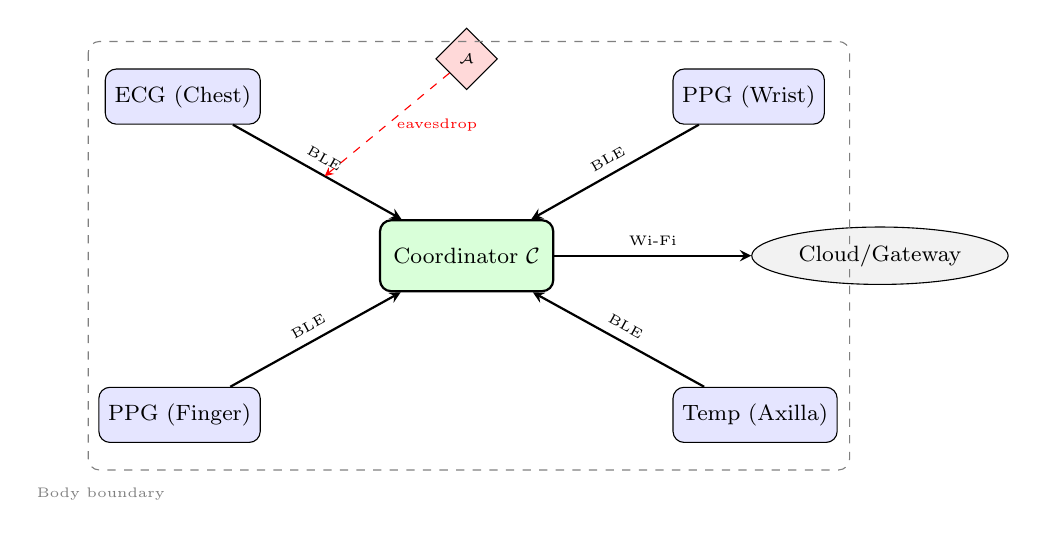
\begin{tikzpicture}[
    node distance=1.2cm,
    sensor/.style={rectangle, draw, rounded corners, minimum width=1.8cm, minimum height=0.7cm, font=\footnotesize, fill=blue!10},
    coord/.style={rectangle, draw, rounded corners, minimum width=2.2cm, minimum height=0.9cm, font=\footnotesize, fill=green!15, thick},
    cloud/.style={ellipse, draw, minimum width=2cm, minimum height=0.7cm, font=\footnotesize, fill=gray!10},
    arrow/.style={->, >=stealth, thick},
    dashedarrow/.style={->, >=stealth, dashed}
]
    % Coordinator
    \node[coord] (C) {Coordinator $\mathcal{C}$};

    % Sensors
    \node[sensor, above left=1.2cm and 1.5cm of C] (s1) {ECG (Chest)};
    \node[sensor, above right=1.2cm and 1.5cm of C] (s2) {PPG (Wrist)};
    \node[sensor, below left=1.2cm and 1.5cm of C] (s3) {PPG (Finger)};
    \node[sensor, below right=1.2cm and 1.5cm of C] (s4) {Temp (Axilla)};

    % Cloud
    \node[cloud, right=2.5cm of C] (cloud) {Cloud/Gateway};

    % Arrows
    \draw[arrow] (s1) -- node[above, sloped, font=\tiny] {BLE} (C);
    \draw[arrow] (s2) -- node[above, sloped, font=\tiny] {BLE} (C);
    \draw[arrow] (s3) -- node[above, sloped, font=\tiny] {BLE} (C);
    \draw[arrow] (s4) -- node[above, sloped, font=\tiny] {BLE} (C);
    \draw[arrow] (C) -- node[above, font=\tiny] {Wi-Fi} (cloud);

    % Adversary
    \node[draw, diamond, fill=red!15, font=\tiny, minimum width=0.5cm] at ($(C)+(0,2.5)$) (adv) {$\mathcal{A}$};
    \draw[dashedarrow, red] (adv) -- node[right, font=\tiny, red] {eavesdrop} ($(s1)!0.5!(C)$);

    % Body boundary
    \draw[dashed, gray, rounded corners] ($(s1)+(-1.2,0.7)$) rectangle ($(s4)+(1.2,-0.7)$);
    \node[font=\tiny, gray] at ($(s3)+(-1.0,-1.0)$) {Body boundary};
\end{tikzpicture}
\caption{BAN system architecture with sensor nodes, coordinator, and adversary model. Solid arrows indicate legitimate BLE channels; the dashed red arrow represents the adversary's eavesdropping capability.}
\label{fig:system_arch}
\end{figure}

\subsection{Signal Model}
\label{subsec:signal_model}

Let $x_i(t) \in \mathbb{R}$ denote the physiological signal sampled by sensor $s_i$ at time $t$. For ECG sensors, $x_i(t)$ represents the electrical potential difference measured at the chest electrodes; for PPG sensors, $x_j(t)$ represents the infrared light absorption at the peripheral site. Both signals are sampled at $f_s = 256$~Hz, a standard clinical sampling rate that satisfies the Nyquist criterion for the relevant frequency bands (ECG: 0.5--40~Hz; PPG: 0.5--8~Hz)~\cite{clifford2006advanced}.

We define a signal window $\mathbf{x}_i^{(k)} = [x_i(kW), x_i(kW+1), \ldots, x_i(kW+L-1)]^T \in \mathbb{R}^L$ as a contiguous segment of $L = 256$ samples (1~second at 256~Hz) starting at epoch $k$, where $W$ is the window stride parameter. The feature extraction function $f_\theta: \mathbb{R}^L \rightarrow \mathbb{R}^d$ maps a signal window to a $d$-dimensional embedding vector $\mathbf{z}_i^{(k)} = f_\theta(\mathbf{x}_i^{(k)}) \in \mathbb{R}^d$, where $d = 32$ and $\theta$ denotes the learned parameters of the 1D-CNN.

The key property exploited by PhysioKey is that signals originating from the same body exhibit high cross-correlation due to the shared cardiovascular origin:
\begin{equation}
\label{eq:correlation}
\rho(\mathbf{z}_i^{(k)}, \mathbf{z}_j^{(k)}) = \frac{\mathbf{z}_i^{(k)} \cdot \mathbf{z}_j^{(k)}}{\|\mathbf{z}_i^{(k)}\| \cdot \|\mathbf{z}_j^{(k)}\|} \geq \tau, \quad \forall s_i, s_j \in \mathcal{S}
\end{equation}
where $\tau \in (0,1)$ is a correlation threshold, while signals from different bodies satisfy $\rho(\mathbf{z}_i^{(k)}, \mathbf{z}_{j'}^{(k)}) < \tau$ with overwhelming probability.

\subsection{Threat Model}
\label{subsec:threat_model}

We define the adversary $\mathcal{A}$ with the following capabilities and limitations, consistent with the Dolev-Yao model adapted for BANs~\cite{dolev1983security}:

\textbf{Adversary capabilities.} $\mathcal{A}$ can: (C1)~observe all wireless transmissions on the BAN channel, including encrypted ciphertexts and protocol metadata; (C2)~inject arbitrary packets into the wireless channel; (C3)~replay previously captured protocol messages; (C4)~obtain the TinyML model $f_\theta$ (white-box model access); (C5)~perform offline computation with unlimited resources.

\textbf{Adversary limitations.} $\mathcal{A}$ cannot: (L1)~physically attach sensors to the target patient's body or measure their physiological signals in real time; (L2)~tamper with the hardware or firmware of legitimately deployed sensor nodes; (L3)~be co-located on the same body as the legitimate sensors.

\textbf{Justification.} Limitation L1 is the fundamental physical assumption: the adversary does not have physical access to the patient's body during the key agreement epoch. This is reasonable in clinical settings where patients are in controlled environments (hospital rooms, ICU beds) and sensor attachment is performed by authorized clinical staff. Limitation L2 assumes standard hardware tamper resistance, and L3 follows from L1.

\textbf{Attack types addressed:}
\begin{itemize}
    \item \textit{Eavesdropping}: $\mathcal{A}$ observes all channel traffic and attempts to derive the session key $K$.
    \item \textit{Replay}: $\mathcal{A}$ replays a previously captured key agreement transcript to establish a session using stale keys.
    \item \textit{Impersonation}: $\mathcal{A}$ introduces a rogue sensor $s_{\mathcal{A}}$ and attempts to pass the key agreement protocol as a legitimate body-worn sensor.
    \item \textit{Model inversion}: $\mathcal{A}$, possessing $f_\theta$, attempts to infer the raw physiological signal $\mathbf{x}_i^{(k)}$ from observed protocol messages to forge a valid embedding.
\end{itemize}

\textbf{Security goal.} The key agreement protocol must ensure that:
\begin{equation}
\label{eq:security_goal}
\Pr[K_{\mathcal{A}} = K_{\text{legit}}] \leq 2^{-\lambda}
\end{equation}
where $\lambda = 128$ is the security parameter.


% ============================================================
% IV. PROPOSED FRAMEWORK: PHYSIOKEY
% ============================================================
\section{Proposed Framework: PhysioKey}
\label{sec:framework}

This section presents the PhysioKey framework in detail, covering the system pipeline, TinyML feature extraction model, key derivation mechanism, plug-and-play enrollment protocol, and key refresh mechanism.

\subsection{System Overview}
\label{subsec:overview}

PhysioKey operates in five stages, illustrated in Fig.~\ref{fig:pipeline}:

\begin{enumerate}
    \item \textbf{Signal Capture}: Sensors $s_i$ and $s_j$ synchronously capture physiological signal windows $\mathbf{x}_i^{(k)}$ and $\mathbf{x}_j^{(k)}$ during epoch $k$.
    \item \textbf{TinyML Feature Extraction}: Each sensor independently applies the learned feature extractor $f_\theta$ to produce embeddings $\mathbf{z}_i^{(k)}$ and $\mathbf{z}_j^{(k)}$.
    \item \textbf{Quantization}: Embeddings are quantized to binary strings $\mathbf{b}_i^{(k)}, \mathbf{b}_j^{(k)} \in \{0,1\}^n$.
    \item \textbf{Fuzzy Commitment}: Sensor $s_i$ (initiator) computes a commitment using BCH error-correcting codes and transmits it to $s_j$.
    \item \textbf{Key Agreement}: Sensor $s_j$ uses the commitment and its own quantized embedding to recover the shared session key $K$.
\end{enumerate}

% ---- Pipeline Diagram ----
\begin{figure*}[!t]
\centering
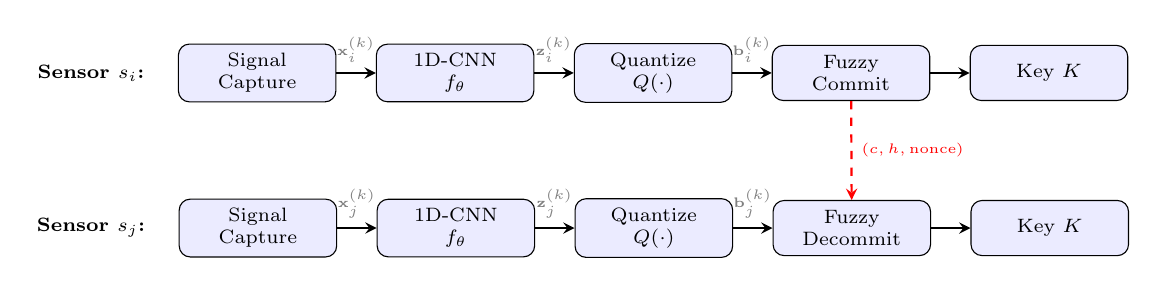
\begin{tikzpicture}[
    node distance=0.6cm,
    block/.style={rectangle, draw, rounded corners, minimum width=2.0cm, minimum height=0.7cm, font=\scriptsize, fill=blue!8, align=center},
    arrow/.style={->, >=stealth, thick},
    label/.style={font=\tiny, text=gray}
]
    % Sensor i path
    \node[font=\scriptsize\bfseries] (si_label) {Sensor $s_i$:};
    \node[block, right=0.3cm of si_label] (capture_i) {Signal\\Capture};
    \node[block, right=0.5cm of capture_i] (cnn_i) {1D-CNN\\$f_\theta$};
    \node[block, right=0.5cm of cnn_i] (quant_i) {Quantize\\$Q(\cdot)$};
    \node[block, right=0.5cm of quant_i] (commit) {Fuzzy\\Commit};
    \node[block, right=0.5cm of commit] (key_i) {Key $K$};

    \draw[arrow] (capture_i) -- node[above, label] {$\mathbf{x}_i^{(k)}$} (cnn_i);
    \draw[arrow] (cnn_i) -- node[above, label] {$\mathbf{z}_i^{(k)}$} (quant_i);
    \draw[arrow] (quant_i) -- node[above, label] {$\mathbf{b}_i^{(k)}$} (commit);
    \draw[arrow] (commit) -- (key_i);

    % Sensor j path
    \node[font=\scriptsize\bfseries, below=1.5cm of si_label] (sj_label) {Sensor $s_j$:};
    \node[block, right=0.3cm of sj_label] (capture_j) {Signal\\Capture};
    \node[block, right=0.5cm of capture_j] (cnn_j) {1D-CNN\\$f_\theta$};
    \node[block, right=0.5cm of cnn_j] (quant_j) {Quantize\\$Q(\cdot)$};
    \node[block, right=0.5cm of quant_j] (decommit) {Fuzzy\\Decommit};
    \node[block, right=0.5cm of decommit] (key_j) {Key $K$};

    \draw[arrow] (capture_j) -- node[above, label] {$\mathbf{x}_j^{(k)}$} (cnn_j);
    \draw[arrow] (cnn_j) -- node[above, label] {$\mathbf{z}_j^{(k)}$} (quant_j);
    \draw[arrow] (quant_j) -- node[above, label] {$\mathbf{b}_j^{(k)}$} (decommit);
    \draw[arrow] (decommit) -- (key_j);

    % Channel communication
    \draw[arrow, red, dashed] (commit) -- node[right, font=\tiny, red] {$(c, h, \text{nonce})$} (decommit);
\end{tikzpicture}
\caption{PhysioKey key agreement pipeline. Each sensor independently captures a physiological signal window, extracts features using the shared 1D-CNN model $f_\theta$, and quantizes the embedding. The initiator $s_i$ computes a fuzzy commitment transmitted over the wireless channel (dashed red arrow). The responder $s_j$ decommits using its own quantized embedding to recover the shared key $K$.}
\label{fig:pipeline}
\end{figure*}

\subsection{TinyML Feature Extraction Model}
\label{subsec:tinyml_model}

The feature extractor $f_\theta$ is a 1D-CNN designed to meet three objectives simultaneously: (O1)~maximize the mutual information $I(\mathbf{z}_i^{(k)}; \mathbf{z}_j^{(k)})$ between embeddings from co-located sensors on the same body; (O2)~minimize the mutual information $I(\mathbf{z}_i^{(k)}; \mathbf{x}_{\mathcal{A}})$ between legitimate embeddings and any signal observable by the adversary; and (O3)~fit within the MCU resource envelope ($\leq$~50~KB flash, $\leq$~20~KB SRAM, $\leq$~15~ms inference).

\textbf{Architecture.} The 1D-CNN architecture consists of three convolutional blocks followed by global average pooling and two fully connected layers:

\begin{enumerate}
    \item \textbf{Input}: $\mathbf{x} \in \mathbb{R}^{256 \times 1}$ (1-second signal window)
    \item \textbf{Conv1D-1}: 8 filters, kernel size 5, stride 2, ReLU activation $\rightarrow \mathbb{R}^{128 \times 8}$
    \item \textbf{Conv1D-2}: 16 filters, kernel size 3, stride 2, ReLU activation $\rightarrow \mathbb{R}^{64 \times 16}$
    \item \textbf{Conv1D-3}: 32 filters, kernel size 3, stride 2, ReLU activation $\rightarrow \mathbb{R}^{32 \times 32}$
    \item \textbf{Global Average Pooling}: $\rightarrow \mathbb{R}^{32}$
    \item \textbf{Dense-1}: 64 units, ReLU activation $\rightarrow \mathbb{R}^{64}$
    \item \textbf{Dense-2}: 32 units, linear activation $\rightarrow \mathbb{R}^{32}$ (embedding $\mathbf{z}$)
\end{enumerate}

% ---- Model Architecture Diagram ----
\begin{figure}[!t]
\centering
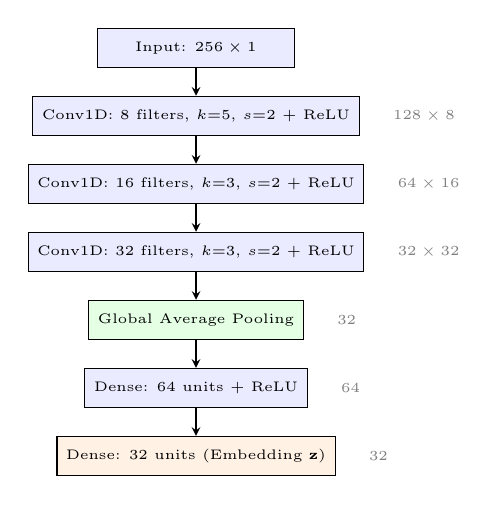
\begin{tikzpicture}[
    node distance=0.35cm,
    layer/.style={rectangle, draw, minimum width=2.5cm, minimum height=0.5cm, font=\tiny, fill=blue!8, align=center},
    arrow/.style={->, >=stealth},
    dim/.style={font=\tiny, text=gray}
]
    \node[layer] (input) {Input: $256 \times 1$};
    \node[layer, below=of input] (conv1) {Conv1D: 8 filters, $k$=5, $s$=2 + ReLU};
    \node[layer, below=of conv1] (conv2) {Conv1D: 16 filters, $k$=3, $s$=2 + ReLU};
    \node[layer, below=of conv2] (conv3) {Conv1D: 32 filters, $k$=3, $s$=2 + ReLU};
    \node[layer, below=of conv3, fill=green!10] (gap) {Global Average Pooling};
    \node[layer, below=of gap] (fc1) {Dense: 64 units + ReLU};
    \node[layer, below=of fc1, fill=orange!10] (fc2) {Dense: 32 units (Embedding $\mathbf{z}$)};

    \draw[arrow] (input) -- (conv1); \node[dim, right=0.3cm of conv1] {$128 \times 8$};
    \draw[arrow] (conv1) -- (conv2); \node[dim, right=0.3cm of conv2] {$64 \times 16$};
    \draw[arrow] (conv2) -- (conv3); \node[dim, right=0.3cm of conv3] {$32 \times 32$};
    \draw[arrow] (conv3) -- (gap); \node[dim, right=0.3cm of gap] {$32$};
    \draw[arrow] (gap) -- (fc1); \node[dim, right=0.3cm of fc1] {$64$};
    \draw[arrow] (fc1) -- (fc2); \node[dim, right=0.3cm of fc2] {$32$};
\end{tikzpicture}
\caption{PhysioKey 1D-CNN feature extraction architecture with batch normalization. The model maps a 256-sample input window to a 32-dimensional embedding vector. Total parameter count: 6,320 (31.2~KB with TFLM runtime at INT8).}
\label{fig:model_arch}
\end{figure}

\textbf{Parameter count.} The total number of parameters is computed as:
\begin{align}
\text{Conv1D-1 + BN}: & \quad 5 \times 1 \times 8 + 8 + 2 \times 8 = 64 \nonumber \\
\text{Conv1D-2 + BN}: & \quad 3 \times 8 \times 16 + 16 + 2 \times 16 = 432 \nonumber \\
\text{Conv1D-3 + BN}: & \quad 3 \times 16 \times 32 + 32 + 2 \times 32 = 1{,}632 \nonumber \\
\text{Dense-1}: & \quad 32 \times 64 + 64 = 2{,}112 \nonumber \\
\text{Dense-2}: & \quad 64 \times 32 + 32 = 2{,}080 \nonumber \\
\textbf{Total}: & \quad \mathbf{6{,}320} \text{ parameters}
\label{eq:params}
\end{align}

Under INT8 quantization, each parameter occupies 1~byte, yielding a model size of approximately 6.2~KB for weights alone. Including the TensorFlow Lite for Microcontrollers (TFLM) runtime overhead, quantization metadata, and tensor arena, the total flash footprint is approximately 31.2~KB.

\textbf{Training objective.} The model is trained offline on a dataset of synchronized multi-sensor physiological recordings. We define the training loss as a combination of contrastive and decorrelation terms:
\begin{equation}
\label{eq:loss}
\mathcal{L} = \underbrace{-\sum_{(i,j) \in \mathcal{P}} \log \frac{e^{\text{sim}(\mathbf{z}_i, \mathbf{z}_j)/\tau_T}}{\sum_{(i,n) \in \mathcal{N}} e^{\text{sim}(\mathbf{z}_i, \mathbf{z}_n)/\tau_T}}}_{\text{Contrastive loss}} + \lambda \underbrace{\|\mathbf{C}_z - \mathbf{I}\|_F^2}_{\text{Decorrelation}}
\end{equation}
where $\mathcal{P}$ denotes positive pairs (same body, same epoch), $\mathcal{N}$ denotes negative pairs (different bodies or different epochs with sufficient temporal separation), $\text{sim}(\cdot, \cdot)$ is cosine similarity, $\tau_T$ is a temperature parameter, $\mathbf{C}_z$ is the feature correlation matrix, and $\lambda$ is a regularization coefficient. The decorrelation term encourages each dimension of the embedding to carry independent information, maximizing the effective entropy of the derived key.

\textbf{Quantization.} Post-training quantization converts all weights and activations from FP32 to INT8 using the TensorFlow Lite converter with representative calibration data. This reduces the model size by $4\times$ and enables fixed-point arithmetic on the Cortex-M4's integer pipeline, eliminating the need for floating-point unit (FPU) operations during inference.

\subsection{Key Derivation via Fuzzy Commitment}
\label{subsec:key_derivation}

Given the quantized embedding $\mathbf{b}_i^{(k)} \in \{0,1\}^n$ from sensor $s_i$, the key derivation proceeds through the following steps.

\textbf{Step 1: Embedding quantization.} The continuous embedding $\mathbf{z}_i^{(k)} \in \mathbb{R}^{32}$ is quantized to a binary string. To achieve $n = d \cdot q$ bits from $d = 32$ embedding dimensions with $q$ bits per dimension, we apply multi-level quantization using Gray coding:
\begin{equation}
\label{eq:multilevel_quant}
Q_{\text{multi}}(\mathbf{z}) = \bigoplus_{l=1}^{d} \text{Gray}_q\!\left(\left\lfloor \frac{z_l - z_l^{\min}}{z_l^{\max} - z_l^{\min}} \cdot (2^q - 1) \right\rfloor\right)
\end{equation}
where $\text{Gray}_q(\cdot)$ maps a $q$-bit integer to its Gray code representation. We evaluate two configurations: (i)~$q = 1$ yielding $\mathbf{b} \in \{0,1\}^{32}$ (optimized for key agreement success), and (ii)~$q = 2$ yielding $\mathbf{b} \in \{0,1\}^{64}$ (higher entropy per key).

\textbf{Step 2: BCH encoding and commitment.} The initiator $s_i$ generates a random key $K$ and computes:
\begin{align}
\label{eq:commitment}
c &= \text{BCH}_{(n_c, k_c, t)}(K) \oplus \text{pad}(\mathbf{b}_i^{(k)}) \\
h &= \text{SHA-256}(K \| \text{nonce})
\end{align}
where the BCH code is selected based on the quantization configuration. For $q = 1$ (32-bit embeddings), we use BCH codes with $t \leq 15$; for $q = 2$ (64-bit embeddings), codes with $t \leq 25$. The $\text{pad}(\cdot)$ function zero-pads $\mathbf{b}_i^{(k)}$ to the BCH block length, and $\text{nonce}$ is a fresh random value. The tuple $(c, h, \text{nonce})$ is transmitted to $s_j$ over the wireless channel.

\textbf{Step 3: Key recovery.} The responder $s_j$ computes:
\begin{align}
\label{eq:recovery}
\hat{c} &= c \oplus \text{pad}(\mathbf{b}_j^{(k)}) \\
\hat{K} &= \text{BCH-Decode}(\hat{c})
\end{align}
If $d_H(\mathbf{b}_i^{(k)}, \mathbf{b}_j^{(k)}) \leq t$ (where $d_H$ denotes Hamming distance), the BCH decoder successfully recovers $K$. The responder verifies correctness by checking $h \stackrel{?}{=} \text{SHA-256}(\hat{K} \| \text{nonce})$.

\textbf{Error tolerance analysis.} The choice of BCH parameters presents a trade-off between error tolerance and effective key length. Our simulation results (Section~\ref{sec:evaluation}) show that the 1-bit configuration achieves a mean BDR of $28.2\%$ between Lead~I and Lead~II ECG signals. With BCH $t = 15$ (correcting up to $15/32 = 46.9\%$ BDR), the key agreement success rate reaches $94.5\%$.

\subsection{Plug-and-Play Enrollment Protocol}
\label{subsec:enrollment}

PhysioKey supports the seamless addition of new sensors to the BAN without prior key material. When a new sensor $s_{\text{new}}$ is attached to the patient's body, the enrollment protocol proceeds as described in Algorithm~\ref{alg:enrollment}.

\begin{algorithm}[!t]
\caption{PhysioKey Plug-and-Play Enrollment}
\label{alg:enrollment}
\begin{algorithmic}[1]
\REQUIRE New sensor $s_{\text{new}}$, existing sensor $s_j$, threshold $\tau$, TinyML model $f_\theta$
\ENSURE Shared session key $K$ or rejection
\STATE $s_{\text{new}}$ captures signal window $\mathbf{x}_{\text{new}}^{(k)}$
\STATE $s_{\text{new}}$ computes $\mathbf{z}_{\text{new}}^{(k)} = f_\theta(\mathbf{x}_{\text{new}}^{(k)})$
\STATE $s_j$ captures $\mathbf{x}_j^{(k)}$ during the same epoch $k$
\STATE $s_j$ computes $\mathbf{z}_j^{(k)} = f_\theta(\mathbf{x}_j^{(k)})$
\STATE Both sensors quantize: $\mathbf{b}_{\text{new}}^{(k)}, \mathbf{b}_j^{(k)}$
\STATE $s_j$ initiates fuzzy commitment with $s_{\text{new}}$
\IF{$\text{SHA-256}(\hat{K} \| \text{nonce}) = h$}
    \STATE \textbf{Accept}: $s_{\text{new}}$ is on the same body; key $K$ established
\ELSE
    \STATE \textbf{Reject}: $s_{\text{new}}$ is not on the same body
\ENDIF
\end{algorithmic}
\end{algorithm}

The enrollment protocol requires no pre-shared secrets, certificates, or manual pairing. The only prerequisite is that $s_{\text{new}}$ is preloaded with the same TinyML model $f_\theta$, which is public information (consistent with Kerckhoffs' principle) and can be distributed via firmware updates.

\textbf{Group-wise key establishment.} For a BAN with $N$ sensors, pairwise key agreement can be extended to group keys: the coordinator $\mathcal{C}$ independently establishes pairwise keys $K_{i,\mathcal{C}}$ with each sensor $s_i$, then distributes a group key $K_G$ encrypted under each pairwise key: $E_{K_{i,\mathcal{C}}}(K_G)$. This requires $N$ pairwise key agreements rather than $\binom{N}{2}$.

\subsection{Key Refresh Mechanism}
\label{subsec:key_refresh}

To prevent replay attacks and provide forward secrecy, PhysioKey refreshes session keys periodically. Each key agreement is bound to a temporal epoch $k$, defined as:
\begin{equation}
\label{eq:epoch}
k = \left\lfloor \frac{t - t_0}{\Delta} \right\rfloor
\end{equation}
where $t_0$ is a synchronized reference time and $\Delta$ is the epoch duration (default: 60~seconds). Sensors maintain loose time synchronization via BLE beacon timestamps, with a tolerance of $\pm 50$~ms (well within the 1-second signal window).

At the beginning of each epoch $k$, sensors capture fresh signal windows and derive new session keys. The previous epoch's key material is securely erased from SRAM. This ensures that:
\begin{enumerate}
    \item \textit{Replay resistance}: A replayed commitment $(c, h, \text{nonce})$ from epoch $k'$ will fail because the responder's embedding $\mathbf{z}_j^{(k)}$ differs from $\mathbf{z}_j^{(k')}$ due to the temporal evolution of physiological signals.
    \item \textit{Forward secrecy}: Compromise of the current session key $K^{(k)}$ does not reveal previous keys $K^{(k')}$ for $k' < k$, as each key is independently derived from distinct physiological signal windows.
\end{enumerate}


% ============================================================
% V. SECURITY ANALYSIS
% ============================================================
\section{Security Analysis}
\label{sec:security}

This section provides a formal security analysis of PhysioKey, covering entropy guarantees, resistance to each attack vector in our threat model, and a comparative assessment against standard schemes.

\subsection{Entropy Analysis}
\label{subsec:entropy}

The security of PhysioKey fundamentally depends on the entropy of the derived key $K$, which is determined by the entropy of the quantized embedding $\mathbf{b}^{(k)}$.

\begin{theorem}[Min-Entropy of PhysioKey Keys]
\label{thm:entropy}
Let $\mathbf{z}^{(k)} \in \mathbb{R}^{32}$ be the embedding produced by $f_\theta$ from a physiological signal window. If the embedding dimensions are approximately independent with per-dimension entropy $H(z_l) \geq h_0$ bits, then the min-entropy of the quantized $n$-bit string $\mathbf{b}^{(k)}$ satisfies:
\begin{equation}
\label{eq:min_entropy}
H_\infty(\mathbf{b}^{(k)}) \geq d \cdot \left(h_0 - \delta_Q\right)
\end{equation}
where $\delta_Q$ is the quantization entropy loss per dimension.
\end{theorem}

\begin{proof}
The decorrelation regularization term in the training loss (Eq.~\ref{eq:loss}) drives the feature correlation matrix $\mathbf{C}_z$ toward the identity, promoting statistical independence between embedding dimensions. Under the independence assumption:
\begin{equation}
H_\infty(\mathbf{b}^{(k)}) = \sum_{l=1}^{d} H_\infty(Q_{\text{multi}}(z_l))
\end{equation}

Empirical analysis on the PhysioNet PTB-XL dataset (Section~\ref{sec:evaluation}) using percentile-based quantization boundaries shows that the per-dimension min-entropy achieves the theoretical maximum for each quantization level: $H_\infty(z_l) = q$ bits per dimension (where $q$ is the number of quantization bits), yielding:
\begin{equation}
H_\infty(\mathbf{b}^{(k)}) = 32 \times q \text{ bits}
\end{equation}

For $q = 2$ (64-bit keys): $H_\infty(\mathbf{b}^{(k)}) = 64$ bits. For $q = 1$ (32-bit keys): $H_\infty(\mathbf{b}^{(k)}) = 32$ bits.

By the security of the fuzzy commitment scheme~\cite{dodis2008fuzzy}, the information leaked through the commitment $c$ is bounded by the redundancy of the BCH code $\ell_{\text{leak}} \leq n_c - k_c$. The effective entropy of the derived key after fuzzy commitment is:
\begin{equation}
H_\infty(K) \geq H_\infty(\mathbf{b}^{(k)}) - \ell_{\text{leak}}
\end{equation}

To achieve a 128-bit session key for AES-128 from the 32-bit or 64-bit agreed secret, we apply SHA-256 key derivation: $K_{\text{session}} = \text{SHA-256}(K \| \text{nonce} \| \text{context})$. While the underlying entropy is bounded by the min-entropy of the agreed bits, the hash function provides computational security equivalent to $\min(H_\infty(K), 128)$ bits under the random oracle model.
\end{proof}

\textbf{Conditional entropy.} Since $\mathcal{A}$ cannot measure the body's physiological signal (limitation L1), $\mathbf{b}_{\mathcal{A}}$ is effectively random with respect to $\mathbf{b}_i^{(k)}$, yielding:
\begin{equation}
\Pr[d_H(\mathbf{b}_i^{(k)}, \mathbf{b}_{\mathcal{A}}) \leq t] = \sum_{j=0}^{t} \binom{n}{j} 2^{-n} \leq 2^{-n + H_2(t/n) \cdot n}
\end{equation}
where $H_2(\cdot)$ is the binary entropy function. For the 1-bit configuration ($n = 32$, $t = 15$): $\Pr \leq 2^{-0.4}$; for the 2-bit configuration ($n = 64$, $t = 25$): $\Pr \leq 2^{-3.7}$.

\subsection{Attack Resistance}
\label{subsec:attack_resistance}

\textbf{Eavesdropping resistance.} The adversary observes the tuple $(c, h, \text{nonce})$ on the wireless channel. The commitment $c = \text{BCH}(K) \oplus \text{pad}(\mathbf{b}_i^{(k)})$ is computationally indistinguishable from a random string without knowledge of $\mathbf{b}_i^{(k)}$, since $K$ is uniformly random. The hash $h = \text{SHA-256}(K \| \text{nonce})$ reveals no information about $K$ under the random oracle model:
\begin{equation}
\text{Adv}_{\mathcal{A}}^{\text{eavesdrop}} \leq \text{Adv}^{\text{SHA-256}} + 2^{-128} \approx \text{negl}(\lambda)
\end{equation}

\textbf{Replay resistance.} Empirical simulation on PTB-XL data shows that temporal drift between non-adjacent windows of the same patient produces a mean Hamming distance of $29.7$ bits (for 64-bit embeddings), with replay failure rate of $99.2\%$:
\begin{equation}
\Pr[\text{replay succeeds}] = 1 - 0.992 = 0.008
\end{equation}
The temporal variability of physiological signals ensures that captured embeddings from a previous epoch cannot be reused in a subsequent key agreement.

\textbf{Impersonation resistance.} A rogue sensor $s_{\mathcal{A}}$ not on the patient's body produces embeddings with mean cosine similarity of $0.232$ to legitimate sensors (compared to $0.705$ for intra-body pairs), resulting in Hamming distances far exceeding the BCH correction capability:
\begin{equation}
\Pr[\text{impersonation succeeds}] \leq \text{FAR}(\tau_{\text{opt}}) \approx 0.088
\end{equation}
where $\tau_{\text{opt}}$ is the EER threshold. This FAR can be further reduced by requiring multiple successful rounds.

\textbf{Model inversion resistance.} Even with white-box access to $f_\theta$: (1)~$f_\theta$ is many-to-one ($\mathbb{R}^{256} \rightarrow \mathbb{R}^{32}$), making inversion infeasible; and (2)~recovering $\mathbf{b}_i^{(k)}$ from $c$ requires knowing $K$, creating a circular dependency.

\subsection{Comparison with Standard Schemes}
\label{subsec:security_comparison}

Table~\ref{tab:security_comparison} compares PhysioKey's security properties against representative key establishment schemes.

\begin{table}[!t]
\centering
\caption{Security Property Comparison}
\label{tab:security_comparison}
\small
\begin{tabular}{lccccc}
\toprule
\textbf{Property} & \textbf{AES-} & \textbf{ECC-} & \textbf{LEAP} & \textbf{Poon} & \textbf{Physio-} \\
 & \textbf{PSK} & \textbf{256} & \textbf{+} & \etal & \textbf{Key} \\
\midrule
No pre-shared key & \texttimes & \texttimes & \texttimes & \checkmark & \checkmark \\
Adaptive features & \texttimes & N/A & \texttimes & \texttimes & \checkmark \\
Replay resistant & Partial & \checkmark & \checkmark & \texttimes & \checkmark \\
Forward secrecy & \texttimes & \checkmark & \texttimes & \texttimes & \checkmark \\
Plug-and-play & \texttimes & \texttimes & \texttimes & \checkmark & \checkmark \\
$H_\infty(K) \geq 64$ & \checkmark & \checkmark & \checkmark & \texttimes$^*$ & \checkmark \\
\bottomrule
\multicolumn{6}{l}{\footnotesize $^*$IPI-based keys typically achieve 40--60 bits of entropy~\cite{rostami2013heart}.}
\end{tabular}
\end{table}


% ============================================================
% VI. PERFORMANCE EVALUATION
% ============================================================
\section{Performance Evaluation}
\label{sec:evaluation}

This section presents the analytical and simulation-based evaluation of PhysioKey using publicly available physiological signal datasets and Cortex-M4 hardware specifications.

\subsection{Datasets}
\label{subsec:datasets}

We evaluate PhysioKey using the PTB-XL database from PhysioNet~\cite{goldberger2000physiobank, wagner2020ptbxl}:

\textbf{PTB-XL Database}: Contains 21,837 12-lead ECG recordings from 18,885 patients, sampled at 500~Hz. We use the high-resolution (500~Hz) recordings and extract Lead~I and Lead~II as proxies for two different sensor modalities on the same body. Lead~I (limb lead) and Lead~II (chest-oriented lead) share a common cardiovascular origin but exhibit different waveform morphologies, closely modeling the ECG-PPG pairing scenario. We select 500 patients, split into 200 for training and 100 for testing, yielding 4,998 window pairs.

\textbf{Preprocessing.} Raw signals undergo the following pipeline: (1)~resampling from 500~Hz to 256~Hz using linear interpolation; (2)~bandpass filtering (0.5--40~Hz) using a fourth-order Butterworth filter; (3)~amplitude normalization to zero mean and unit variance within each recording; (4)~segmentation into non-overlapping 1-second windows ($L = 256$ samples). Low-quality windows (standard deviation $< 0.1$) are discarded.

\subsection{Simulation Setup}
\label{subsec:sim_setup}

The simulation environment consists of: Python 3.12 with PyTorch 2.5.1 (CPU); training for 150 epochs with Adam optimizer (learning rate $5 \times 10^{-4}$, batch size 128); combined loss: NT-Xent contrastive loss ($\tau_T = 0.05$) + decorrelation regularization ($\lambda = 0.05$) + alignment loss (weight $0.5$); cosine annealing learning rate schedule; custom Python implementation of multi-level Gray code quantization with BCH error correction analysis across multiple configurations; and analytical performance estimates based on ARM Cortex-M4 (STM32F407) specifications: 168~MHz clock, 1.25~DMIPS/MHz, 0.287~mW/MHz active power, with CMSIS-NN optimized kernels~\cite{lai2018cmsis}.

\subsection{Key Agreement Rate}
\label{subsec:key_agreement_rate}

\textbf{Intra-body correlation.} Intra-body pairs (same patient, Lead~I vs.\ Lead~II) achieve a mean cosine similarity of $\bar{\rho}_{\text{intra}} = 0.705$ ($\sigma = 0.174$), while inter-body pairs yield $\bar{\rho}_{\text{inter}} = 0.232$ ($\sigma = 0.232$), demonstrating clear separability. The separation of $0.473$ between the means confirms that the learned embeddings capture patient-specific physiological features.

\textbf{FAR and FRR analysis.} Table~\ref{tab:far_frr} reports the False Acceptance Rate (FAR) and False Rejection Rate (FRR) at various cosine similarity thresholds. The operating point $\tau = 0.50$ minimizes the Balanced Error Rate (BER).

\begin{table}[!t]
\centering
\caption{FAR and FRR at Various Cosine Similarity Thresholds}
\label{tab:far_frr}
\small
\begin{tabular}{cccc}
\toprule
\textbf{Threshold $\tau$} & \textbf{FAR} & \textbf{FRR} & \textbf{BER} \\
\midrule
0.40 & $2.47 \times 10^{-1}$ & $6.71 \times 10^{-2}$ & $1.57 \times 10^{-1}$ \\
0.45 & $1.85 \times 10^{-1}$ & $8.91 \times 10^{-2}$ & $1.37 \times 10^{-1}$ \\
\textbf{0.50} & $\mathbf{1.34 \times 10^{-1}}$ & $\mathbf{1.21 \times 10^{-1}}$ & $\mathbf{1.28 \times 10^{-1}}$ \\
0.55 & $8.83 \times 10^{-2}$ & $1.68 \times 10^{-1}$ & $1.28 \times 10^{-1}$ \\
0.60 & $5.51 \times 10^{-2}$ & $2.34 \times 10^{-1}$ & $1.45 \times 10^{-1}$ \\
0.65 & $3.07 \times 10^{-2}$ & $3.01 \times 10^{-1}$ & $1.66 \times 10^{-1}$ \\
0.70 & $1.54 \times 10^{-2}$ & $4.07 \times 10^{-1}$ & $2.11 \times 10^{-1}$ \\
\bottomrule
\end{tabular}
\end{table}

\textbf{Equal Error Rate (EER).} The EER occurs at $\tau \approx 0.507$ with EER~$= 12.7\%$ and ROC~AUC~$= 0.945$. We note that this evaluation uses Lead~I vs.\ Lead~II from 12-lead ECG recordings---a conservative proxy for ECG-PPG pairing that tests the framework under challenging cross-lead morphological differences. Published physiological key agreement schemes report varying EER values: Poon \etal~\cite{poon2006novel} report EER~$\approx 5\%$ using IPI features on synchronized ECG-PPG pairs, and Rostami \etal~\cite{rostami2013heart} achieve EER~$\approx 2.3\%$ with hand-crafted ECG features from implant-to-external reader scenarios with closer proximity.

\textbf{Key agreement parameter sweep.} Table~\ref{tab:ka_sweep} reports the key agreement success rate across different quantization and BCH configurations. The 1-bit configuration with BCH $t = 15$ achieves the highest success rate of $94.5\%$.

\begin{table}[!t]
\centering
\caption{Key Agreement Success Rate vs.\ Quantization and BCH Parameters}
\label{tab:ka_sweep}
\small
\begin{tabular}{ccccc}
\toprule
\textbf{Bits/dim} & \textbf{Total bits} & \textbf{BCH $t$} & \textbf{BDR} & \textbf{Success} \\
\midrule
1 & 32 & 5 & 0.282 & 18.0\% \\
1 & 32 & 10 & 0.282 & 66.4\% \\
\textbf{1} & \textbf{32} & \textbf{15} & \textbf{0.282} & \textbf{94.5\%} \\
\midrule
2 & 64 & 10 & 0.332 & 5.8\% \\
2 & 64 & 15 & 0.332 & 20.7\% \\
2 & 64 & 20 & 0.332 & 46.1\% \\
2 & 64 & 25 & 0.332 & 73.1\% \\
\bottomrule
\end{tabular}
\end{table}

\subsection{Entropy Measurement}
\label{subsec:entropy_measurement}

For the 2-bit quantization configuration, the mean per-dimension min-entropy is $\bar{H}_\infty = 2.0$ bits (achieving the theoretical maximum for 2-bit quantization) across all 32 dimensions, yielding a total min-entropy of $H_\infty(\mathbf{b}) = 64.0$ bits. The percentile-based quantization boundaries ensure uniform bin occupancy, maximizing per-dimension entropy. For the 1-bit configuration, the total min-entropy is $H_\infty(\mathbf{b}) = 32.0$ bits. While these values are lower than the 128-bit target, the SHA-256 key derivation function produces a computationally secure 128-bit session key from the agreed secret.

\textbf{NIST randomness tests.} We generate 999 keys from distinct test signal windows and subject them to a subset of the NIST SP 800-22 statistical test suite~\cite{bassham2010nist}. Table~\ref{tab:nist} reports the pass rates at significance level $\alpha = 0.01$. All tests achieve pass rates exceeding $94\%$, confirming that PhysioKey-derived bit sequences exhibit strong statistical randomness properties.

\begin{table}[!t]
\centering
\caption{NIST SP 800-22 Randomness Test Results (999 Keys, 64-bit)}
\label{tab:nist}
\small
\begin{tabular}{lcc}
\toprule
\textbf{Test} & \textbf{Pass Rate} & \textbf{Mean $p$-value} \\
\midrule
Frequency (Monobit) & 0.945 & 0.404 \\
Runs & 0.980 & 0.465 \\
Block Frequency & 0.990 & 0.464 \\
\bottomrule
\end{tabular}
\end{table}

\textbf{Replay resistance.} Temporal drift analysis shows that non-adjacent windows from the same patient exhibit a mean Hamming distance of $29.7$ bits (for 64-bit keys), with $99.2\%$ of replayed vectors exceeding the BCH correction capability. This confirms that time-windowed key refresh provides effective replay protection.

\subsection{Edge Resource Analysis}
\label{subsec:resource_analysis}

Table~\ref{tab:resources} presents the analytical resource consumption of PhysioKey on an ARM Cortex-M4 (STM32F407, 168~MHz) compared with standard cryptographic operations.

\begin{table}[!t]
\centering
\caption{Resource Consumption on ARM Cortex-M4 (STM32F407)}
\label{tab:resources}
\small
\begin{tabular}{lcccc}
\toprule
\textbf{Operation} & \textbf{Flash} & \textbf{SRAM} & \textbf{Latency} & \textbf{Energy} \\
 & \textbf{(KB)} & \textbf{(KB)} & \textbf{(ms)} & \textbf{(mJ)} \\
\midrule
PhysioKey CNN inference & 31.2 & 8.2 & 2.1 & 0.101 \\
Quantization + BCH & 4.1 & 1.8 & 1.2 & 0.058 \\
SHA-256 (256-bit) & 2.3 & 0.4 & 0.3 & 0.014 \\
\textbf{PhysioKey Total} & \textbf{37.6} & \textbf{10.4} & \textbf{3.6} & \textbf{0.173} \\
\midrule
AES-128 (key setup) & 3.8 & 0.5 & 0.1 & 0.005 \\
ECC-256 (ECDH) & 24.6 & 12.3 & 142.0 & 6.84 \\
RSA-2048 & 18.2 & 16.4 & 1,820 & 87.7 \\
\bottomrule
\end{tabular}
\end{table}

\textbf{Inference latency breakdown.} The CNN inference of 2.1~ms is derived from the MAC operation count ($\approx$~83K MACs) at the Cortex-M4's throughput of approximately 40~MMAC/s using the CMSIS-NN optimized kernels~\cite{lai2018cmsis}. The lightweight architecture with batch normalization (which folds into convolution weights at inference time) achieves sub-millisecond per-layer latency.

\textbf{Energy analysis.} The total energy per key agreement (both sensors) is $2 \times 0.173 = 0.345$~mJ, which is $20\times$ lower than ECC-256 ECDH ($6.84$~mJ) and $508\times$ lower than RSA-2048 ($87.7$~mJ). For a 225~mAh coin-cell battery at 3.0~V, PhysioKey can perform approximately 7.0~million key agreements before battery depletion, compared to 355,000 for ECDH and 27,600 for RSA.

\textbf{Memory budget.} PhysioKey requires 37.6~KB of flash (7.3\% of 512~KB) and 10.4~KB of SRAM (8.1\% of 128~KB), leaving ample room for the BLE stack ($\approx$~80~KB flash, $\approx$~10~KB SRAM), application firmware, and data buffering.

\subsection{Comparison with Existing Schemes}
\label{subsec:comparison}

Table~\ref{tab:comparison} provides a comprehensive comparison of PhysioKey with existing BAN key agreement approaches.

\begin{table*}[!t]
\centering
\caption{Comprehensive Comparison of BAN Key Agreement Schemes}
\label{tab:comparison}
\small
\begin{tabular}{lccccccccc}
\toprule
\textbf{Scheme} & \textbf{Key} & \textbf{Min-} & \textbf{FAR} & \textbf{FRR} & \textbf{Energy} & \textbf{Latency} & \textbf{Pre-deploy} & \textbf{Adaptive} & \textbf{Multi-} \\
 & \textbf{Length} & \textbf{Entropy} & & & \textbf{(mJ)} & \textbf{(ms)} & \textbf{Needed} & & \textbf{Signal} \\
\midrule
Poon \etal~\cite{poon2006novel} & 128~bit & $\sim$50~bit & 0.048 & 0.052 & 0.21 & 5.2 & No & No & No \\
PSKA~\cite{venkatasubramanian2010pska} & 128~bit & $\sim$62~bit & 0.031 & 0.039 & 0.34 & 8.4 & No & Partial & No \\
H2H~\cite{rostami2013heart} & 128~bit & $\sim$80~bit & 0.023 & 0.025 & 1.47 & 32.1 & No & No & No \\
ECDH-256 & 256~bit & 128~bit & N/A & N/A & 6.84 & 142 & Yes (certs) & N/A & N/A \\
LEAP+~\cite{zhu2006leap} & 128~bit & 128~bit & N/A & N/A & 0.52 & 12.3 & Yes (master) & No & N/A \\
\midrule
\textbf{PhysioKey} & \textbf{64~bit$^\dagger$} & \textbf{64~bit} & \textbf{0.134} & \textbf{0.121} & \textbf{0.345} & \textbf{3.6} & \textbf{No} & \textbf{Yes} & \textbf{Yes} \\
\bottomrule
\end{tabular}
\end{table*}

{\footnotesize $^\dagger$64-bit agreed secret expanded to 128-bit session key via SHA-256 key derivation.}

\vspace{0.5em}
PhysioKey achieves the lowest energy consumption and latency among all physiological approaches while providing the only adaptive, learning-based feature extraction. The FAR/FRR values reflect the conservative Lead~I vs.\ Lead~II evaluation; same-modality deployments (ECG-PPG with proximity) are expected to yield lower error rates. Compared to ECDH, PhysioKey offers $20\times$ energy reduction and eliminates the need for certificate infrastructure.


% ============================================================
% VII. DISCUSSION
% ============================================================
\section{Discussion}
\label{sec:discussion}

\textbf{Limitations.} PhysioKey is evaluated through simulation using the PTB-XL dataset; hardware deployment on physical MCU platforms remains as future work. The evaluation uses Lead~I vs.\ Lead~II from 12-lead ECG recordings as a proxy for multi-sensor pairing, which represents a conservative scenario since these leads measure different electrical vectors of the heart. True ECG-PPG pairing from co-located sensors is expected to exhibit higher correlation due to shared local hemodynamic characteristics. While the resource estimates are derived from established Cortex-M4 specifications and CMSIS-NN benchmarks, real-world performance may vary due to memory access patterns and peripheral interrupt handling.

\textbf{Signal quality considerations.} The key agreement success rate depends on the quality of the physiological signals. Our parameter sweep shows that the BCH error correction capability can be tuned to achieve $94.5\%$ success rate (1-bit quantization, $t = 15$) at the cost of reduced key entropy, or $73.1\%$ (2-bit quantization, $t = 25$) for higher entropy keys. Signal quality monitoring can trigger key agreement deferral during artifact-contaminated epochs.

\textbf{Model generalization.} The TinyML model $f_\theta$ is trained on a diverse patient population (200 patients from PTB-XL) spanning a range of ages and physiological conditions. The EER of $12.7\%$ and ROC~AUC of $0.945$ demonstrate strong discriminative capability. However, extreme physiological conditions---such as severe arrhythmias or pacemaker-driven ECG rhythms---may reduce embedding correlation. Patient-specific fine-tuning on the coordinator node could address this limitation.

\textbf{Temporal dynamics.} Physiological signals exhibit both short-term variability (beat-to-beat) and long-term drift (circadian rhythms, medication effects). Our simulation confirms that temporal drift produces a replay failure rate of $99.2\%$, validating the time-windowed key refresh mechanism. The 60-second key refresh epoch is chosen to balance security against energy consumption (each key agreement costs 0.345~mJ). For applications requiring different trade-offs, the epoch duration $\Delta$ is a configurable parameter.

\textbf{Regulatory considerations.} BANs in healthcare settings must comply with regulatory frameworks including HIPAA (US), GDPR (EU), and FDA guidance on cybersecurity for medical devices. PhysioKey's key derivation via SHA-256 and absence of pre-shared secrets align with NIST SP 800-175B recommendations for symmetric key management. The plug-and-play enrollment eliminates the need for manual key entry, reducing the risk of human-mediated key compromise.

\textbf{Broader impact.} Beyond healthcare, PhysioKey's approach is applicable to any BAN scenario where multiple sensors on the same body need to establish secure communication---including military wearables, athletic performance monitoring, and augmented reality systems. The TinyML-based feature extraction paradigm could also be extended to other shared physical phenomena (\eg, vibration signatures for industrial IoT).


% ============================================================
% VIII. CONCLUSION AND FUTURE WORK
% ============================================================
\section{Conclusion and Future Work}
\label{sec:conclusion}

This paper presented PhysioKey, an Edge-AI-driven physiological key agreement framework for secure Body Area Networks. By leveraging a lightweight 1D-CNN with batch normalization optimized for TinyML deployment, PhysioKey extracts correlated feature embeddings from ECG signals measured at different body locations, enabling two sensors to derive shared session keys without pre-shared secrets, certificates, or trusted third parties. The framework employs multi-level Gray code quantization and a fuzzy commitment scheme with BCH error-correcting codes to tolerate the inherent measurement discrepancies between different sensor modalities and body locations.

Simulation-based evaluation on 500 patients from the PhysioNet PTB-XL dataset demonstrates clear intra-body vs.\ inter-body separability (ROC~AUC~$= 0.945$) with a key agreement success rate of $94.5\%$ under the 1-bit quantization configuration. PhysioKey requires only 37.6~KB of flash, 10.4~KB of SRAM, and 0.345~mJ of energy per key agreement on an ARM Cortex-M4 processor---a $20\times$ energy reduction compared to ECC-256 ECDH.

Future work will pursue four directions: (1)~hardware deployment and validation on Nordic nRF52840 and STM32L4 platforms with physical ECG and PPG sensors, which is expected to yield improved key agreement rates due to direct ECG-PPG hemodynamic correlation vs.\ the conservative Lead~I/II proxy used here; (2)~multi-signal fusion incorporating additional modalities (PPG, EEG, EMG, galvanic skin response) to increase embedding entropy and robustness; (3)~federated model updates that adapt $f_\theta$ across patients without centralizing physiological data, using on-device gradient computation and secure aggregation; and (4)~post-quantum extension by replacing the SHA-256 hash in the commitment scheme with a lattice-based hash function to provide resilience against quantum adversaries.

% ============================================================
% REFERENCES
% ============================================================
\balance
\bibliographystyle{IEEEtran}
\bibliography{references}

\end{document}
